\section{Zielsetzung}
\label{sec:Zielsetzung}

In diesem Versuch soll die Verdampfungswärme von destilliertem Wasser ermittelt werden.
Dafür wird das destillierte Wasser erhitzt und die Temperaturabhängigkeit des Dampfdruckes gemessen. 
Aus der resultierenden Dampfdruckkurve kann anschließend die gesuchte Verdampfungswärme berechnet werden.

\section{Theorie}
\label{sec:Theorie}

Wasser kann, so wie viele andere Stoffe, in drei verschiedenen Phasen vorliegen, nämlich fest, flüssig oder gasförmig.
Welcher dieser drei Zustände angenommen wird, hängt dabei von dem jeweiligen Druck $p$ und der Temperatur $T$ ab.
In \autoref{fig:Zustandsdiagramm} ist qualitativ dargestellt, wann welche Phasen vorliegen.

\begin{figure} [H]
    \centering
    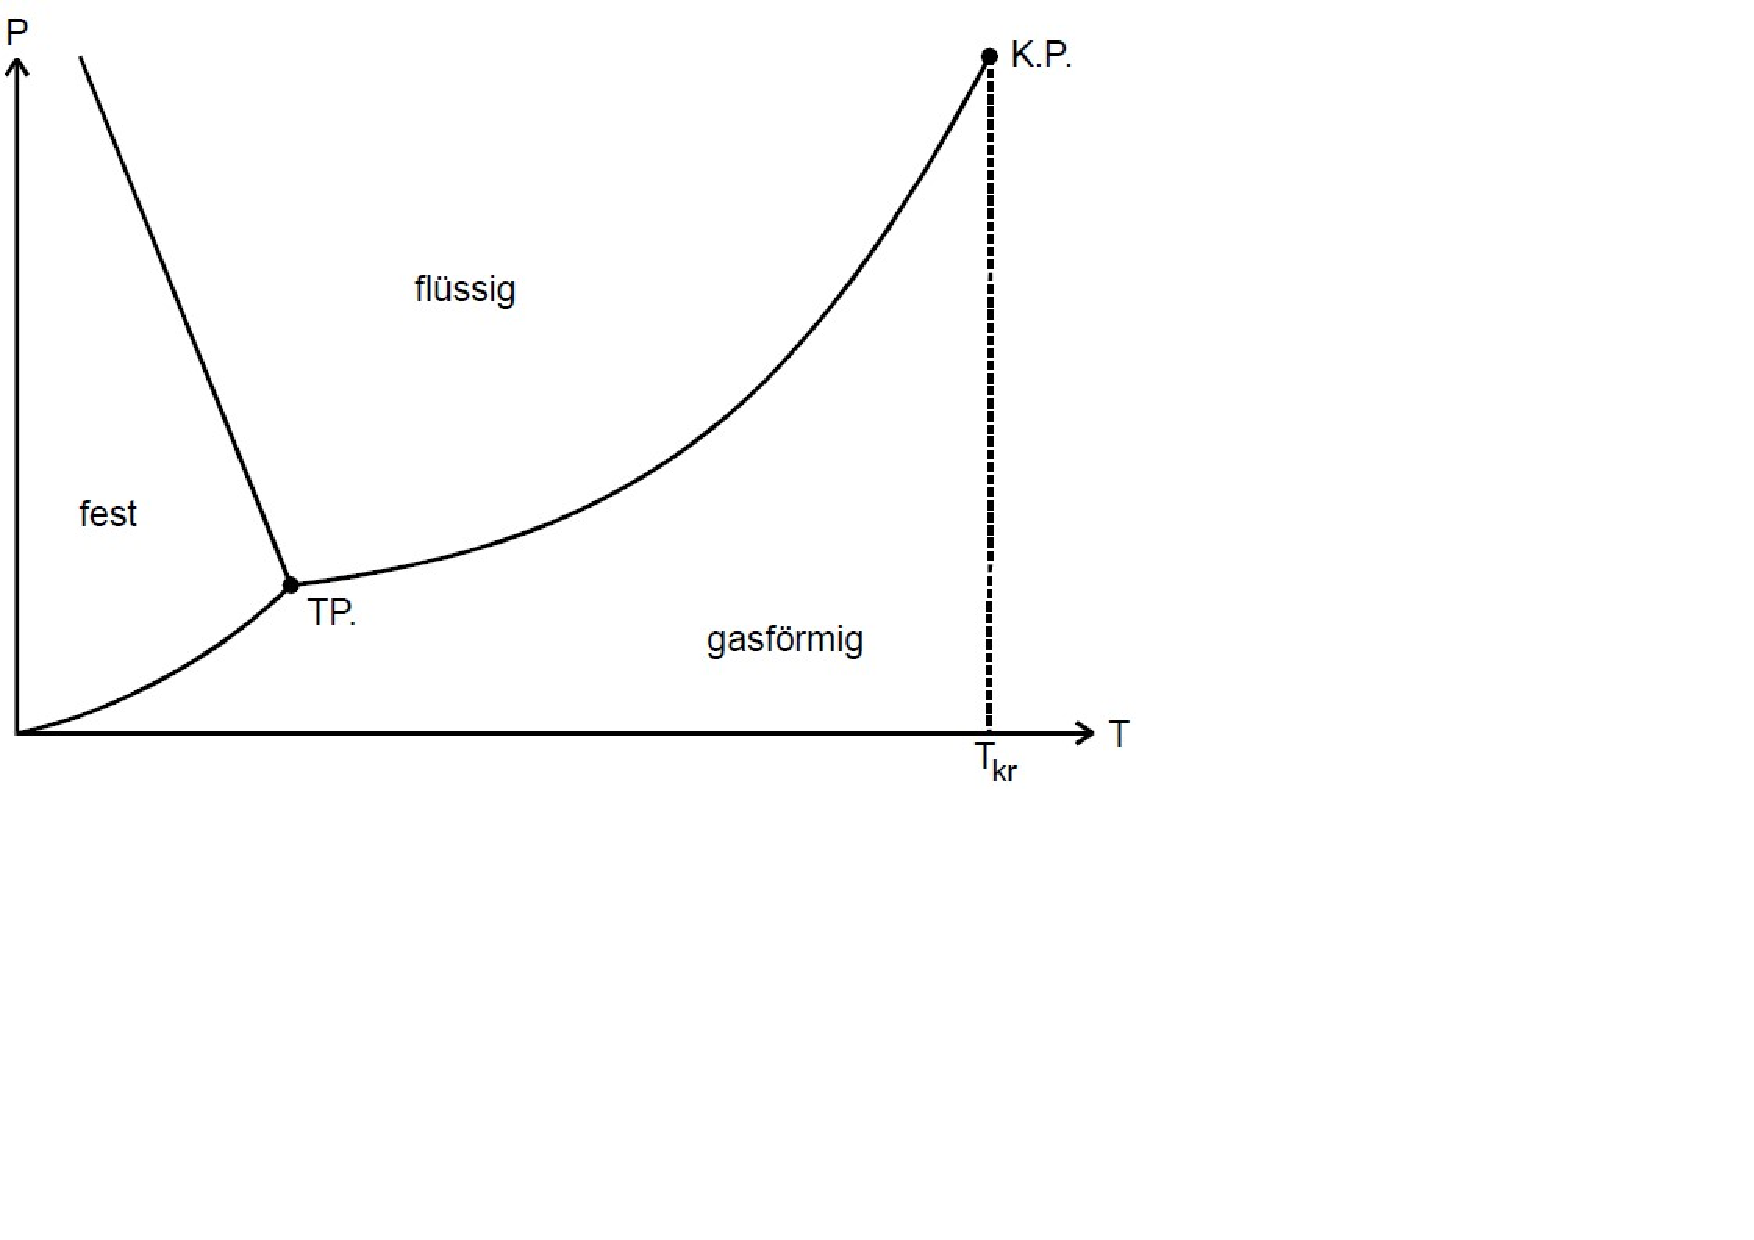
\includegraphics[height=7cm]{content/Bilder/Zustandsdiagramm.pdf}
    \caption{Qualitatives Zustandsdiagramm von Wasser. \cite{v203}}
    \label{fig:Zustandsdiagramm}
\end{figure}

Wasser beginnt zu sieden, wenn es sich nahe dem Übergang zwischen flüssig und gasförmig befindet.
Diese Trennung der Phasen wird durch die sogenannte Dampfdruckkurve beschrieben, hier können die beiden Phasen koexistieren.
Befindet man sich auf der Dampfdruckkurve, dann sind $p$ und $T$ voneinander abhängig.

Ihr Verlauf wird durch die Verdampfungswärme $L$ charakterisiert, dies ist eine stoff- und temperaturabhängige Größe.
Im Bereich der Messung ist $L$ nahezu unabhängig von der Temperatur und kann daher als konstant angenommen werden.
Die Verdampfungswärme beschreibt, wie viel Energie notwendig ist, um eine bestimmte Stoffmenge zu verdampfen.
Genauer betrachtet setzt sich $L$ aus der inneren und äußeren Verdampfungswärme zusammen:

\begin{equation}
    L=L_{\symup{i}}+L_{\symup{a}}
    \label{eq:Verdampfungswärme}
\end{equation}

Dabei beschreibt $L_{\symup{i}}$ die Arbeit zur Überwindung der molekularen Anziehungskräfte, während $L_{\symup{a}}$
für die benötigte Energie steht, um das Volumen des Stoffes zu vergrößern.

Der analytische Verlauf der Dampfdruckkurve wird durch die Clausius-Clapeyronsche Gleichung festgelegt, wobei
$V_{\symup{D}}$ und $V_{\symup{F}}$ für das Volumen vor und nach dem verdampfen stehen:

\begin{equation}
    (V_{\symup{D}}-V_{\symup{F}})\symup{dp}=\frac{L}{T}\symup{dT}
    \label{eq:Clausius-Clapeyronsche Gleichung}
\end{equation}

Nimmt man an, dass $V_{\symup{D}}$ gegenüber $V_{\symup{F}}$ vernachlässigt werden kann, dann
lässt sich $V_{\symup{D}}$ durch die ideale Gasgleichung 

\begin{equation}
    pV=RT
    \label{eq:Ideale Gasgleichung}
\end{equation}

beschreiben. Da $L$, wie bereits erwähnt, als konstant angenommen wird, kann \eqref{eq:Clausius-Clapeyronsche Gleichung}
durch folgende Funktion $p(T)$ gelöst werden:

\begin{equation}
    p(T)=p_0\symup{e}^{-\frac{L}{R}\cdot\frac{1}{T}}.
    \label{eq:Druck}
\end{equation}

Diese Funktion beschreibt also den Verlauf der Dampfdruckkurve und kann zur Bestimmung von $L$ verwendet werden, wenn
der Kurvenverlauf bereits gegeben ist.